\documentclass[tikz,border=3pt]{standalone}
\usepackage{pgfplots}
\pgfplotsset{compat=1.16}
\definecolor{scatterBlue}{HTML}{1F77B4}
\definecolor{scatterOrange}{HTML}{D65F00}
\begin{document}
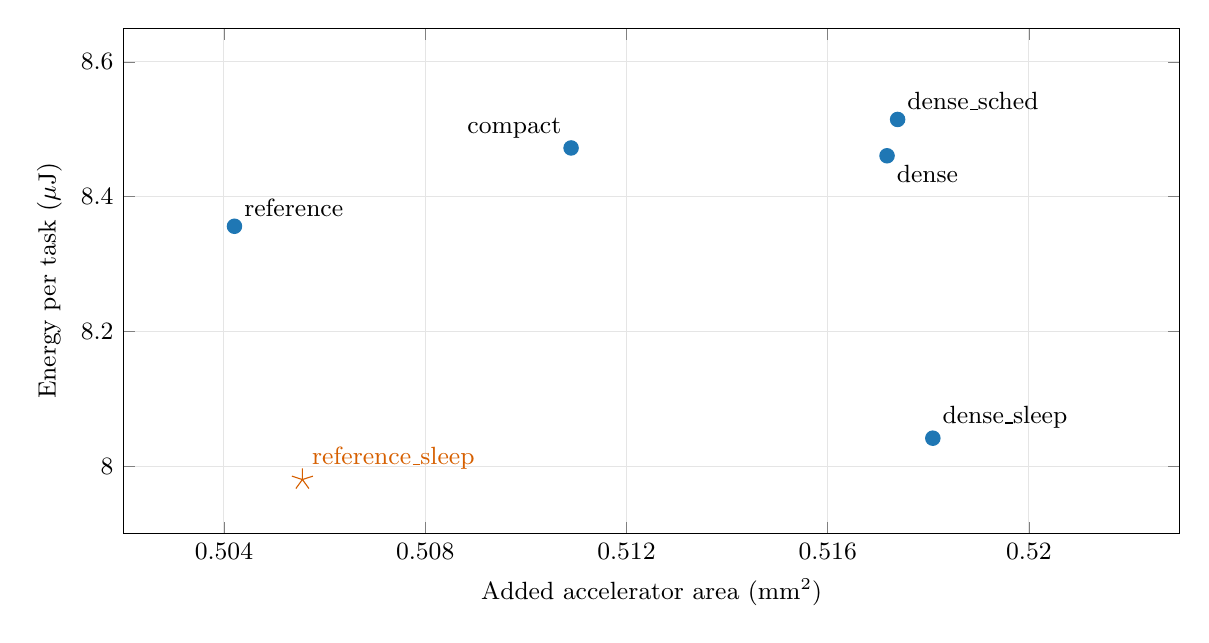
\begin{tikzpicture}
\begin{axis}[width=15cm,height=8cm,xmin=0.502,xmax=0.523,ymin=7.90,ymax=8.65,xlabel={Added accelerator area (mm$^2$)},ylabel={Energy per task ($\mu$J)},scaled x ticks=false,xtick={0.504,0.508,0.512,0.516,0.520},xticklabel style={/pgf/number format/fixed,/pgf/number format/precision=3},grid=major,grid style={gray!20},tick label style={font=\small},label style={font=\small},clip=false]
\addplot[only marks,mark=*,mark size=2.6pt,color=scatterBlue] coordinates {(0.504210,8.3561) (0.510900,8.4723) (0.517180,8.4607) (0.518090,8.0416) (0.517390,8.5146)};
\addplot[only marks,mark=star,mark size=4pt,color=scatterOrange] coordinates {(0.505560,7.9802)};
\node[anchor=south west,font=\small] at (axis cs:0.504210,8.3561) {reference};
\node[anchor=south east,font=\small] at (axis cs:0.510900,8.4723) {compact};
\node[anchor=north west,font=\small] at (axis cs:0.517180,8.4607) {dense};
\node[anchor=south west,font=\small] at (axis cs:0.518090,8.0416) {dense\_sleep};
\node[anchor=south west,font=\small] at (axis cs:0.517390,8.5146) {dense\_sched};
\node[anchor=south west,font=\small,text=scatterOrange] at (axis cs:0.505560,7.9802) {reference\_sleep};
\end{axis}
\end{tikzpicture}
\end{document}